\documentclass[a4paper]{article}
\usepackage{cmap}
\usepackage[utf8]{inputenc}
\usepackage[T2A]{fontenc}
\usepackage[english,russian]{babel} 
\usepackage[left=15mm, top=15mm, right=15mm, bottom=30mm, nohead, nofoot]{geometry}
\usepackage{array}
\usepackage{blindtext}  % рыба-текст
\usepackage{graphicx}  % изобржаения
\usepackage{float} % плавающие объекты
\usepackage{wrapfig}  % изобржаения
\usepackage{tikz} % графика
\usepackage{mdframed} % рамки
\usepackage{xcolor} % определение цветов
\usepackage{nicefrac} % красивые дроби
\usepackage{cancel} % сокращение
\usepackage{amsmath,amsfonts,amssymb} % математический пакет
\usepackage{hyperref}  % гиперссылки
\usepackage{fancybox,fancyhdr} % хедер и футер
\usepackage{listings} % код
\usepackage[skip=2pt]{caption} % расстояние между подписью и картинкой
\pagestyle{fancy}
\fancyhf{}
\fancyhead[L]{Лабораторная работа №1}
\fancyhead[R]{\textit{Моделирование линейных динамических систем}}
\fancyfoot[C]{\thepage}
\headsep=4mm
\footskip=13mm
\setlength{\parindent}{0em}
\setlength{\parsep}{0em}
\setlength{\headheight}{12pt}
\setlength{\topmargin}{-38pt}

\definecolor{urlcolor}{HTML}{3454D1}
\definecolor{linkcolor}{HTML}{3454D1}
\hypersetup{
    pdfstartview=FitH,
    linkcolor=linkcolor,
    urlcolor=urlcolor,
    colorlinks=true,
    pdftitle={Лабораторная работа №1},
    pdfauthor={Овчинников П.А.}
}

\definecolor{strings}{rgb}{0,0.6,0}
\definecolor{comments}{rgb}{0,0.3,0}
\definecolor{numbers}{rgb}{0.5,0.5,0.5}
\definecolor{keywords}{rgb}{0.09,0.61,0.95}
\definecolor{background}{rgb}{0.97,0.97,0.97}
\lstdefinestyle{codestyle}{
    backgroundcolor=\color{background},
    commentstyle=\color{comments},
    keywordstyle=\color{keywords},
    stringstyle=\color{strings},
    numberstyle=\tiny\color{numbers},
    basicstyle=\ttfamily\footnotesize,
    breakatwhitespace=false,
    breaklines=true,
    captionpos=b,
    inputencoding=utf8,
    keepspaces=true,
    numbers=left,
    numbersep=5pt,
    showspaces=false,
    showstringspaces=false,
    showtabs=false,
    tabsize=2,
    extendedchars=true,
    literate=
    {а}{{\cyra}}1
    {б}{{\cyrb}}1
    {в}{{\cyrv}}1
    {г}{{\cyrg}}1
    {д}{{\cyrd}}1
    {е}{{\cyre}}1
    {ж}{{\cyrzh}}1
    {з}{{\cyrz}}1
    {и}{{\cyri}}1
    {й}{{\cyrishrt}}1
    {к}{{\cyrk}}1
    {л}{{\cyrl}}1
    {м}{{\cyrm}}1
    {н}{{\cyrn}}1
    {о}{{\cyro}}1
    {п}{{\cyrp}}1
    {р}{{\cyrr}}1
    {с}{{\cyrs}}1
    {т}{{\cyrt}}1
    {у}{{\cyru}}1
    {ф}{{\cyrf}}1
    {х}{{\cyrh}}1
    {ц}{{\cyrc}}1
    {ч}{{\cyrch}}1
    {ш}{{\cyrsh}}1
    {щ}{{\cyrshch}}1
    {ъ}{{\cyrhrdsn}}1
    {ы}{{\cyrery}}1
    {ь}{{\cyrsftsn}}1
    {э}{{\cyrerev}}1
    {ю}{{\cyryu}}1
    {я}{{\cyrya}}1
    {А}{{\CYRA}}1
    {Б}{{\CYRB}}1
    {В}{{\CYRV}}1
    {Г}{{\CYRG}}1
    {Д}{{\CYR96}}1
    {Е}{{\CYRE}}1
    {Ж}{{\CYRZH}}1
    {З}{{\CYRZ}}1
    {И}{{\CYRI}}1
    {Й}{{\CYRISHRT}}1
    {К}{{\CYRK}}1
    {Л}{{\CYRL}}1
    {М}{{\CYRM}}1
    {Н}{{\CYRN}}1
    {О}{{\CYRO}}1
    {П}{{\CYRP}}1
    {Р}{{\CYRR}}1
    {С}{{\CYRS}}1
    {Т}{{\CYRT}}1
    {У}{{\CYRU}}1
    {Ф}{{\CYRF}}1
    {Х}{{\CYRH}}1
    {Ц}{{\CYRC}}1
    {Ч}{{\CYRCH}}1
    {Ш}{{\CYRSH}}1
    {Щ}{{\CYRSHCH}}1
    {Ъ}{{\CYRHRDSN}}1
    {Ы}{{\CYRERY}}1
    {Ь}{{\CYRSFTSN}}1
    {Э}{{\CYREREV}}1
    {Ю}{{\CYRYU}}1
    {Я}{{\CYRYA}}1
}
\lstset{style=codestyle}

\addto\captionsrussian{
  \renewcommand{\contentsname}
    {\centering Содержание}
}
\newcommand{\addsection}[1]{
    \phantomsection
    \addcontentsline{toc}{section}{#1}
    \section*{\centering #1}
}
\newcommand{\addsubsection}[1]{
    \phantomsection
    \addcontentsline{toc}{subsection}{#1}
    \subsection*{\centering #1}
}
\newcommand{\addsubsubsection}[1]{
    \phantomsection
    \addcontentsline{toc}{subsubsection}{#1}
    \subsubsection*{\centering #1}
}

\newmdenv[
    leftmargin = 0.5em,
    skipabove = 0.5em,
    skipbelow = 0.5em,
    linewidth = 1pt,
    rightline = false,
    topline = false,
    bottomline = false
]{quotebox}

\newlength{\tempheight}
\newcommand{\Let}{
\mathbin{\text{\settoheight{\tempheight}{\mathstrut}\raisebox{0.4\pgflinewidth}{
\tikz[baseline=0.5ex,line cap=round,line join=round] \draw (0,0) --++ (0.3em,0) --++ (0,2.3ex) --++ (-0.3em,0);
}}}}
\newcommand*\squared[1]{\tikz[baseline=(char.base)]{
            \node[shape=rectangle,draw,inner sep=4pt] (char) {#1};}}
\newcommand*\msquared[1]{\tikz[baseline=(char.base)]{
            \node[shape=rectangle,draw,inner sep=4pt] (char) {$\displaystyle #1$};}}
\newcommand\argmax[1]{\underset{#1}{\text{argmax}}}
\renewcommand\max[1]{\underset{#1}{\text{max}}}
\newcommand{\at}{\biggr\rvert}
\newcommand{\shiftright}[3]{\makebox[#2][r]{\makebox[#1][l]{#3}}}
\newcommand{\e}{\;\text{e}}
\let\oldint\int
\def\int{\oldint\limits}
\DeclareRobustCommand{\divby}{%
  \mathrel{\vbox{\baselineskip.65ex\lineskiplimit0pt\hbox{.}\hbox{.}\hbox{.}}}%
}

\newcommand\NB{\textbf{N\kern-0.32em\textcolor{red}{B}}}

\begin{document}
\begin{titlepage}
    \begin{center}
    \includegraphics[width=0.18\textwidth]{~/Изображения/itmo_logo.png}\\[10pt]
        Федеральное государственное автономное образовательное \\ учреждение высшего образования \\[6pt]
        САНКТ-ПЕТЕРБУРГСКИЙ НАЦИОНАЛЬНЫЙ \\ ИССЛЕДОВАТЕЛЬСКИЙ УНИВЕРСИТЕТ ИТМО \\[16pt]
        Факультет систем управления и робототехники \vfill
        {\large Лабораторная работа №1} \\[0.5em]
        {\large\textbf{\MakeUppercase{Моделирование линейных динамических систем}}}\\[0.5em]
        Вариант №12
    \end{center}\vfill
    \begin{flushright}
        Студент: Овчинников П.А.\\
        Поток: ЛСАУ R22 бак 4.1.1 \\[0.5em]
        Преподаватели: Лопарев А.В.\\Золотаревич В.П.
    \end{flushright}\vfill
    \begin{center}
        {\small Санкт-Петербург \\ 2024}
    \end{center}
\end{titlepage}
\setcounter{page}{2}
\tableofcontents\newpage
\textbf{Цель работы:} ознакомление с пакетом прикладных программ Simulink и основными прёмами моделирования линейных динамических систем.

\addsection{Исследование модели вход-выход}
\addsubsection{Порядок выполнения работы}
\begin{itemize}
    \item Построить схему моделирования линейной динамической системы в соответствии с параметрами:
    $$n = 2, \quad a_0=0.12, \quad a_1=1, \quad b_0=0.1, \quad b_1=2, \quad b_2=0.$$
    \item Смоделировать систему с нулевыми начальными условиями при следующих видах входного воздействия:
    $$u = 1(t),\quad u=2\sin t.$$
    Вывести графики $u(t)$ и $y(t)$. Продолжительность интервала наблюдения выбрать самостоятельно.
    \item Смоделировать свободное движение системы с нулевым входным воздействием и следующими начальными условиями:
    $$y(0)=1, \quad \dot{y}(0)=0.$$
    Вывести график $y(t)$.
\end{itemize}

%MARK: №1
\addsubsection{Выполнение работы}
Математическая модель линейной стационарной системы может быть представлена в виде скалярного дифференциального уравнения $n$-го порядка и имеет вид:
$$y^{(n)}+a_{n-1}y^{(n-1)}+\ldots+a_1y^{(1)}+a_0y = b_mu^{(m)}+b_{m-1}u^{(m-1)}+\ldots+b_1u^{(1)}+b_0u,$$
где $y$ --- выходная переменная, $u$ --- входной сигнал, $n$ --- порядок системы, $m$ --- порядок производной выходной переменной, в явном виде зависящей от $u (m \leqslant n)$, $a_j$, $b_j$ --- постоянные коэффициенты. Используя заданные в таблице параметры, сформируем дифференциальное уравнение 2-го порядка:
$$\ddot{y}+\dot{y}+0.12y= 2\dot{u}+0.1u.$$
Заменим дифференцирование его оператором $p = \nicefrac{d}{dt}$ и выразим выходную переменную со старшей степенью $p$:
$$p^2y+py+0.12y = 2pu+0.1u \quad \Rightarrow \quad p^2y = 2pu+0.1u-py-0.12y.$$
Теперь разделим обе части уравнения на $p^2$ и сгруппируем слагаемые:
$$y = \frac{2u}{p}+\frac{0.1u}{p^2}-\frac{y}{p}-\frac{0.12y}{p^2} \quad \Rightarrow \quad y = \frac{1}{p^2}(0.1u-0.12y)+\frac{1}{p}(2u-y).$$
Таким образом выход представлен в виде сумм сигналов с разными коэффициентами, проинтегрированных два и один раз соответственно. Составим схему, ориентируясь на математическую модель:
\begin{figure}[H]
    \centering
    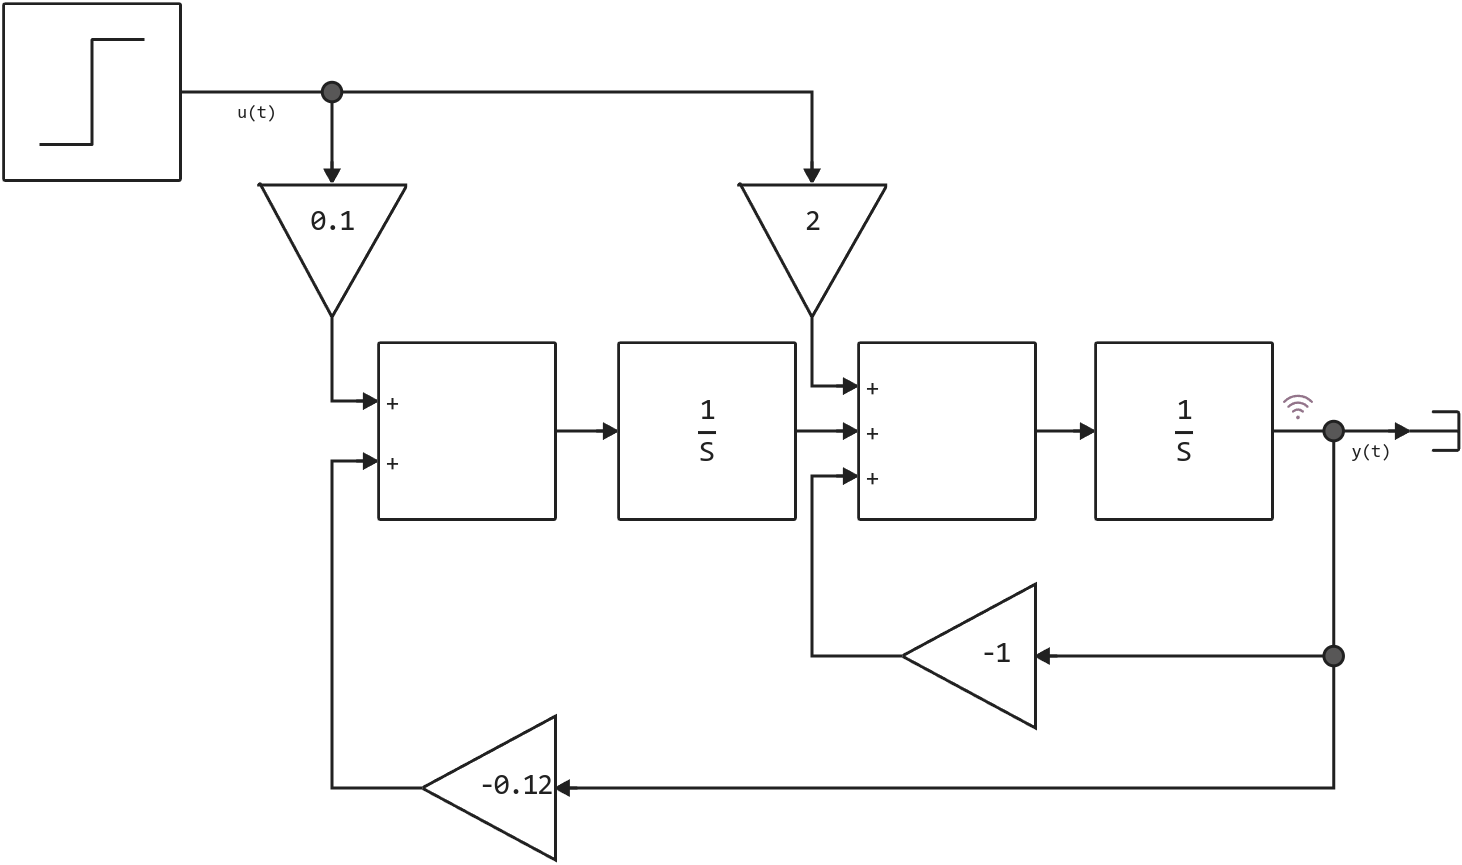
\includegraphics[height=0.23\textheight]{sources/task1_1t_model.png}
    \caption*{Схема моделирования линейной динамической системы с сигналом $u=1(t)$}
\end{figure}
К отчёту приложён файл \href{run:sources}{\texttt{task1.engee}}, содержащий схему моделирования линейной динамической системы в самой полной своей версии. Симуляция проведена в среде моделирования и симуляции \href{https://start.engee.com/}{Engee}.\\[0.5em]
Построим графики $u(t)$ и $y(t)$ (продолжительность интервала наблюдения выбрана $[0, 60]$):
\begin{figure}[H]
    \centering
    \begin{minipage}{0.4\textwidth}
        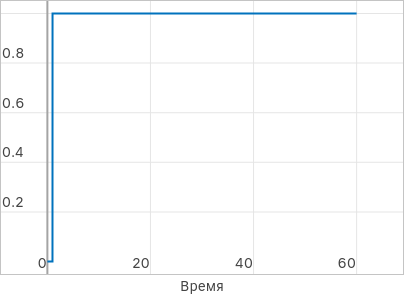
\includegraphics[width=\textwidth]{sources/task1_1t_u.png}
        \caption*{График $u(t)$ для $u=1(t)$}
    \end{minipage}
    \hspace{2em}
    \begin{minipage}{0.4\textwidth}
        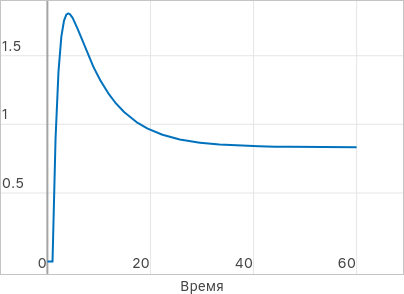
\includegraphics[width=\textwidth]{sources/task1_1t_y.png}
        \caption*{График $y(t)$ для $u=1(t)$}
    \end{minipage}
\end{figure}
Таким же образом строим схему моделирования системы уже с сигналом $u=2\sin{t}$:
\begin{figure}[H]
    \centering
    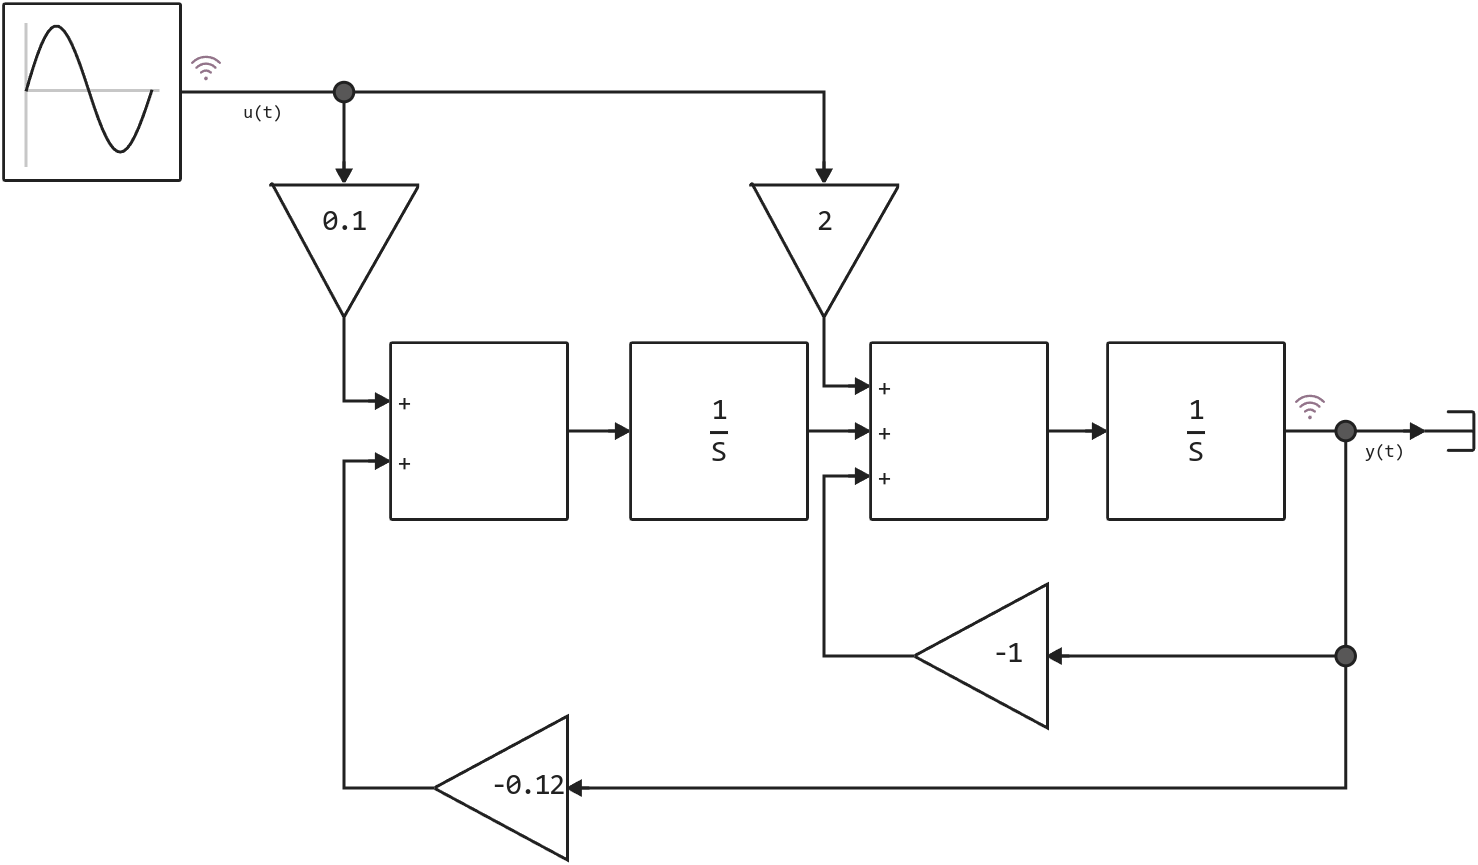
\includegraphics[height=0.23\textheight]{sources/task1_2sint_model.png}
    \caption*{Схема моделирования линейной динамической системы с сигналом $u=2\sin{t}$}
\end{figure}
И вновь построим графики $u(t)$ и $y(t)$:
\begin{figure}[H]
    \centering
    \begin{minipage}{0.4\textwidth}
        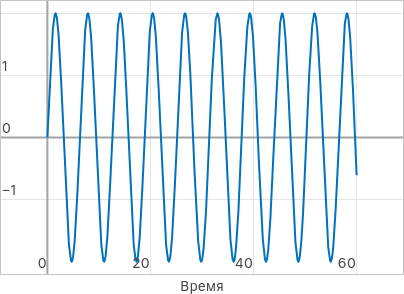
\includegraphics[width=\textwidth]{sources/task1_2sint_u.png}
        \caption*{График $u(t)$ для $u=2\sin{t}$}
    \end{minipage}
    \hspace{2em}
    \begin{minipage}{0.4\textwidth}
        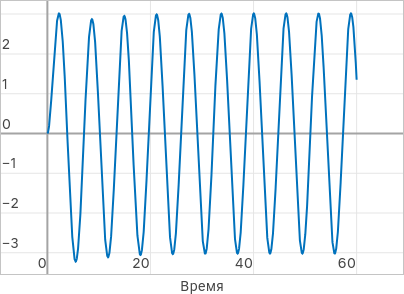
\includegraphics[width=\textwidth]{sources/task1_2sint_y.png}
        \caption*{График $y(t)$ для $u=2\sin{t}$}
    \end{minipage}
\end{figure}
Чтобы смоделировать свободное движение системы, установим $y(0)=1$ и $\dot{y}(0)=0$ и определим начальные условия интеграторов. Обозначим для удобства выходные сигналы интеграторов через $q_1$ и $q_2$. Из схемы моделирования видно, что:
$$\dot{y} = \dot{q}_1 = q_2 + 2u - y \quad \Rightarrow \quad q_2 = \dot{y} + 2u - y.$$
Подставим начальные значения $\dot{y}(0)$ и $y(0)$ ($u(0)$ = 0, т.к. входное воздействие нулевое) и получим начальное значение второго интегратора:
$$q_2(0) = \dot{y}(0) + 2u(0) - y(0) = 0 + 2\cdot0 - 1 = -1.$$
При этом начальное значение первого интегратора выходит из $\dot{y} = \dot{q}_1$:
$$\dot{y} = \dot{q}_1 \quad\Rightarrow\quad y = q_1 \quad\Rightarrow\quad q_1(0) = y(0) = 1.$$
В схеме моделирования зададим интеграторам начальные значения и уберём входное воздействие — таким образом получим схему моделирования свободного движения системы:
\begin{figure}[H]
    \centering
    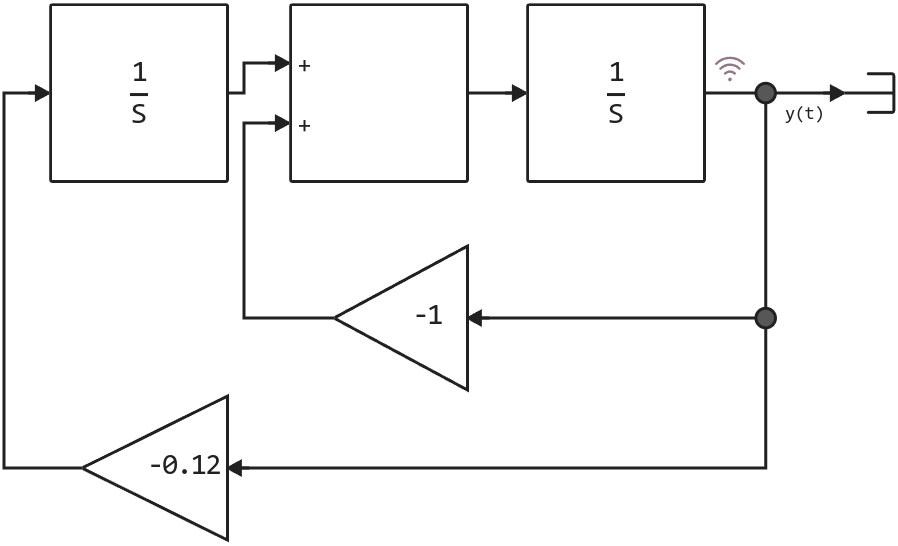
\includegraphics[height=0.15\textheight]{sources/task1_free_model.png}
    \caption*{Схема моделирования свободного движения линейной динамической системы}
\end{figure}
График $y(t)$ в таком случае будет выглядеть так:
\begin{figure}[H]
    \centering
    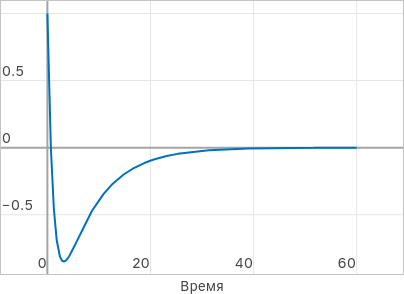
\includegraphics[width=0.4\textwidth]{sources/task1_free_y.png}
    \caption*{График $y(t)$ при свободном движении системы}
\end{figure}

\newpage
\addsection{Исследование модели вход-состояние-выход}
\addsubsection{Порядок выполнения работы}
\begin{itemize}
    \item Построить схему моделирования линейной динамической системы в соответствии с параметрами:
    $$n = 3, \quad A=\begin{vmatrix}
        0 & -15 & 2 \\ 1 & -0.5 & 0 \\ 0 & 0 & -0.25
    \end{vmatrix}, \quad B=\begin{vmatrix}
        2 \\ 0 \\ 0.5
    \end{vmatrix}, \quad C^T=\begin{vmatrix}
        0 \\ 2 \\ 0.25
    \end{vmatrix}.$$
    \item Смоделировать систему с нулевым начальным значением состояния при таких видах входного воздействия:
    $$u = 1(t),\quad u=2\sin t.$$
    Вывести графики $u(t)$ и $y(t)$.
    \item Смоделировать свободное движение системы со следующими начальными условиями:
    $$x_1(0)=-5, \quad x_2(0)=0.5, \quad x_3(0)=0$$
    Вывести график $y(t)$.
\end{itemize}

%MARK: №2
\addsubsection{Выполнение работы}
Математическая модель линейной стационарной системы может быть представлена в виде $n$ дифференциальных уравнений первого порядка. Обычно систему записывают в компактной векторно-матричной форме:
$$\begin{cases}
    \dot{x} = Ax + Bu, \\
    y = Cx,
\end{cases}$$
где $A$ --- $n \times n$ матрица постоянных коэффициентов, $B$ --- $n$-мерный вектор-столбец постоянных коэффициентов, $C$ --- $n$-мерный вектор-строка постоянных коэффициентов, а $x$ --- $n$-мерный вектор состояния. Как раз все три матрицы нам даны по условию задания. Запишем, как в нашем случае будет описываться система:
$$\begin{cases}
    \dot{x}_1 &= -15x_2 + 2x_3 + 2u \\
    \dot{x}_2 &= x_1 - 0.5x_2 \\
    \dot{x}_3 &= -0.25x_3 + 0.5u \\
    y &= 2x_2 + 0.25x_3
\end{cases}$$
В таком случае схема, моделирующая систему, будет выглядеть следующим образом:
\begin{figure}[H]
    \centering
    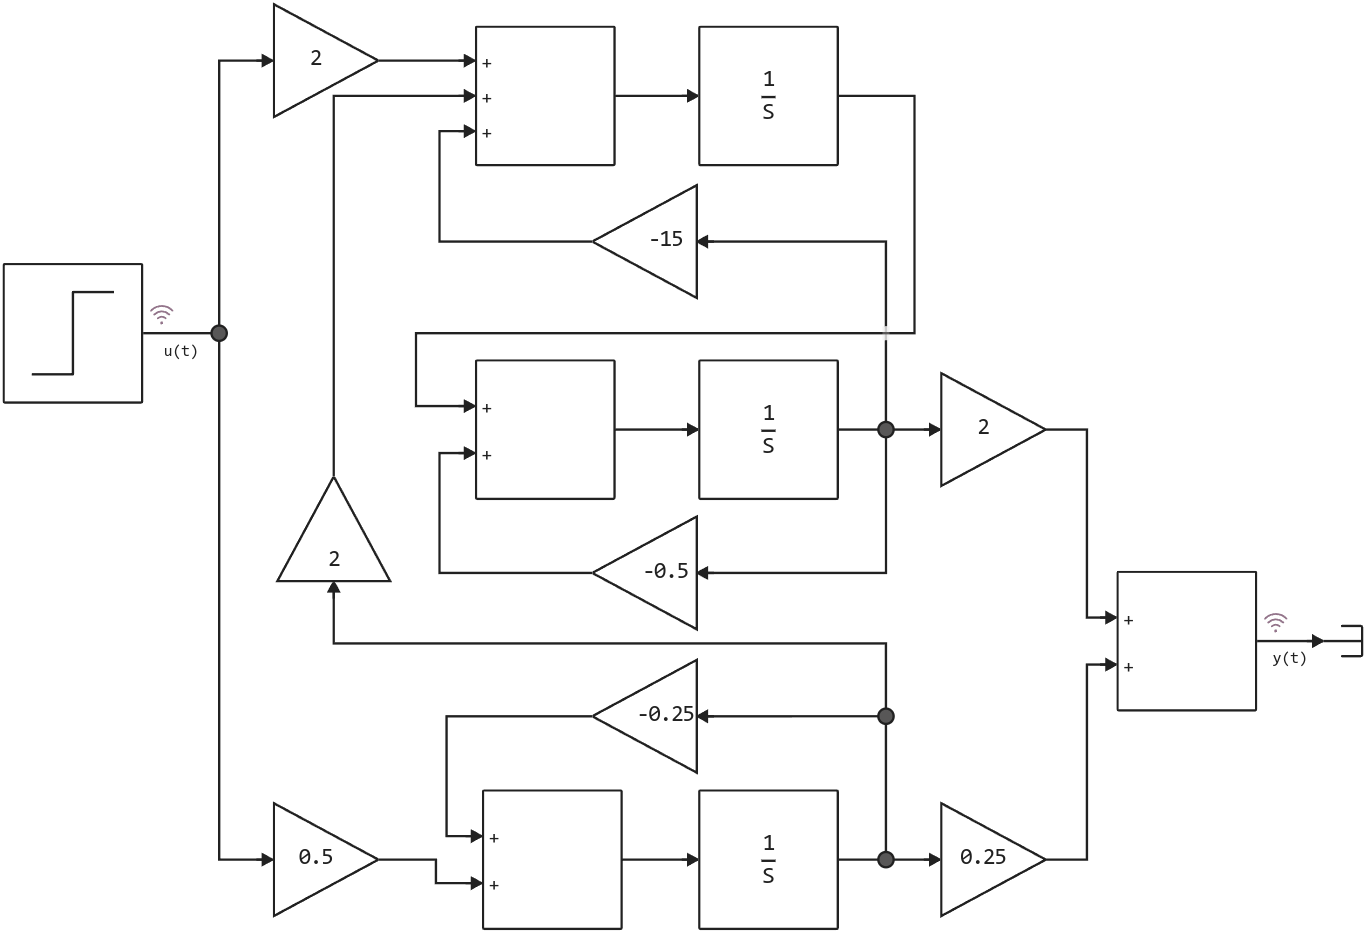
\includegraphics[height=0.27\textheight]{sources/task2_1t_model.png}
    \caption*{Схема моделирования линейной динамической системы с сигналом $u=1(t)$}
\end{figure}
К отчёту также приложён файл \href{run:sources}{\texttt{task2.engee}}, который можно использовать в среде моделирования и симуляции \href{https://start.engee.com/}{Engee}, чтобы восстановить схему в самой полной своей версии.\newpage
Теперь построим графики $u(t)$ и $y(t)$ (продолжительность интервала наблюдения выбрана $[0, 30]$):
\begin{figure}[H]
    \centering
    \begin{minipage}{0.4\textwidth}
        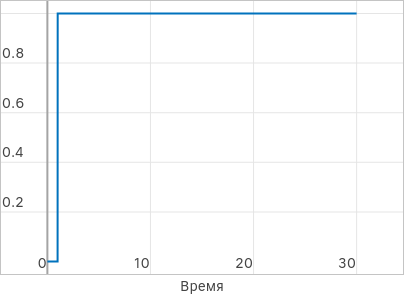
\includegraphics[width=\textwidth]{sources/task2_1t_u.png}
        \caption*{График $u(t)$ для $u=1(t)$}
    \end{minipage}
    \hspace{2em}
    \begin{minipage}{0.4\textwidth}
        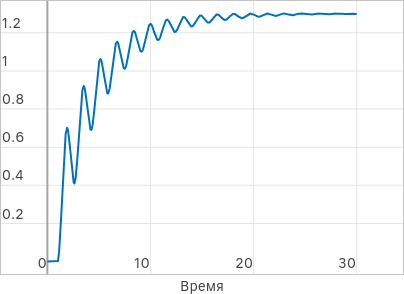
\includegraphics[width=\textwidth]{sources/task2_1t_y.png}
        \caption*{График $y(t)$ для $u=1(t)$}
    \end{minipage}
\end{figure}
Построим схему моделирования системы с сигналом $u=2\sin{t}$. Схема отличается лишь входным сигналом:
\begin{figure}[H]
    \centering
    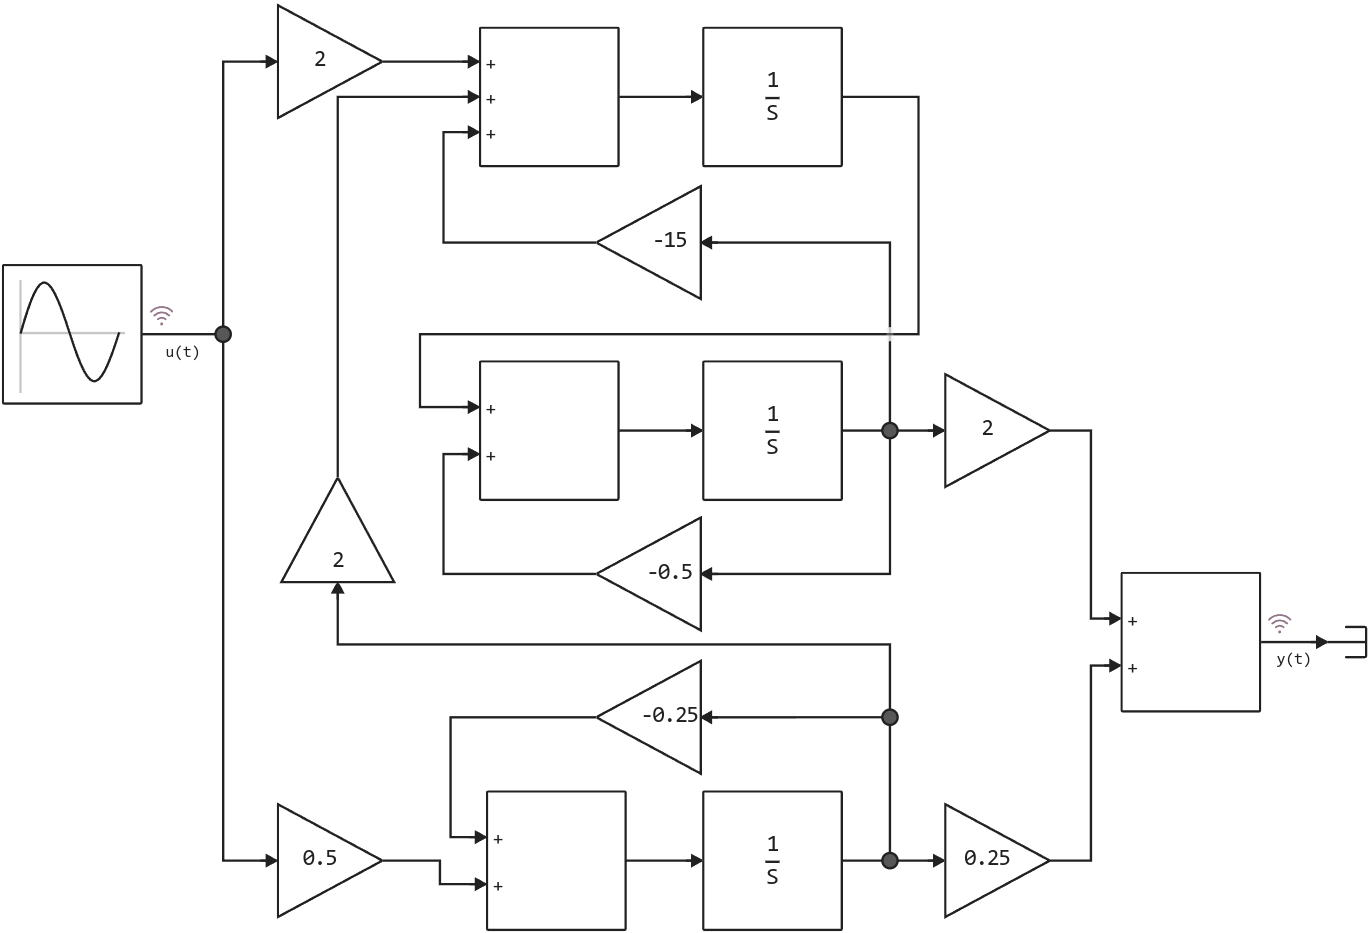
\includegraphics[height=0.27\textheight]{sources/task2_2sint_model.png}
    \caption*{Схема моделирования линейной динамической системы с сигналом $u=2\sin{t}$}
\end{figure}
И приведём графики $u(t)$ и $y(t)$:
\begin{figure}[H]
    \centering
    \begin{minipage}{0.4\textwidth}
        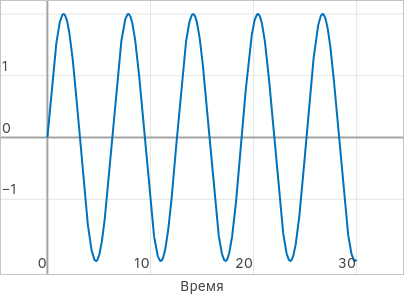
\includegraphics[width=\textwidth]{sources/task2_2sint_u.png}
        \caption*{График $u(t)$ для $u=2\sin{t}$}
    \end{minipage}
    \hspace{2em}
    \begin{minipage}{0.4\textwidth}
        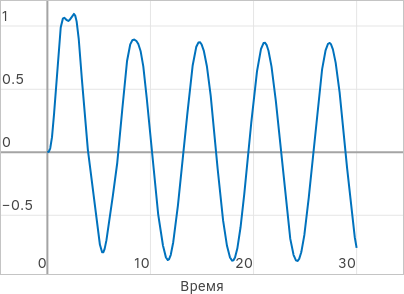
\includegraphics[width=\textwidth]{sources/task2_2sint_y.png}
        \caption*{График $y(t)$ для $u=2\sin{t}$}
    \end{minipage}
\end{figure}
Для моделирования свободного движения системы просто подставим начальные значения состояний $x_1(0)=-5$, $x_2(0)=0.5$, $x_3(0)=0$ в начальные условия на интеграторах в схеме и уберём входное воздействие:
\begin{figure}[H]
    \centering
    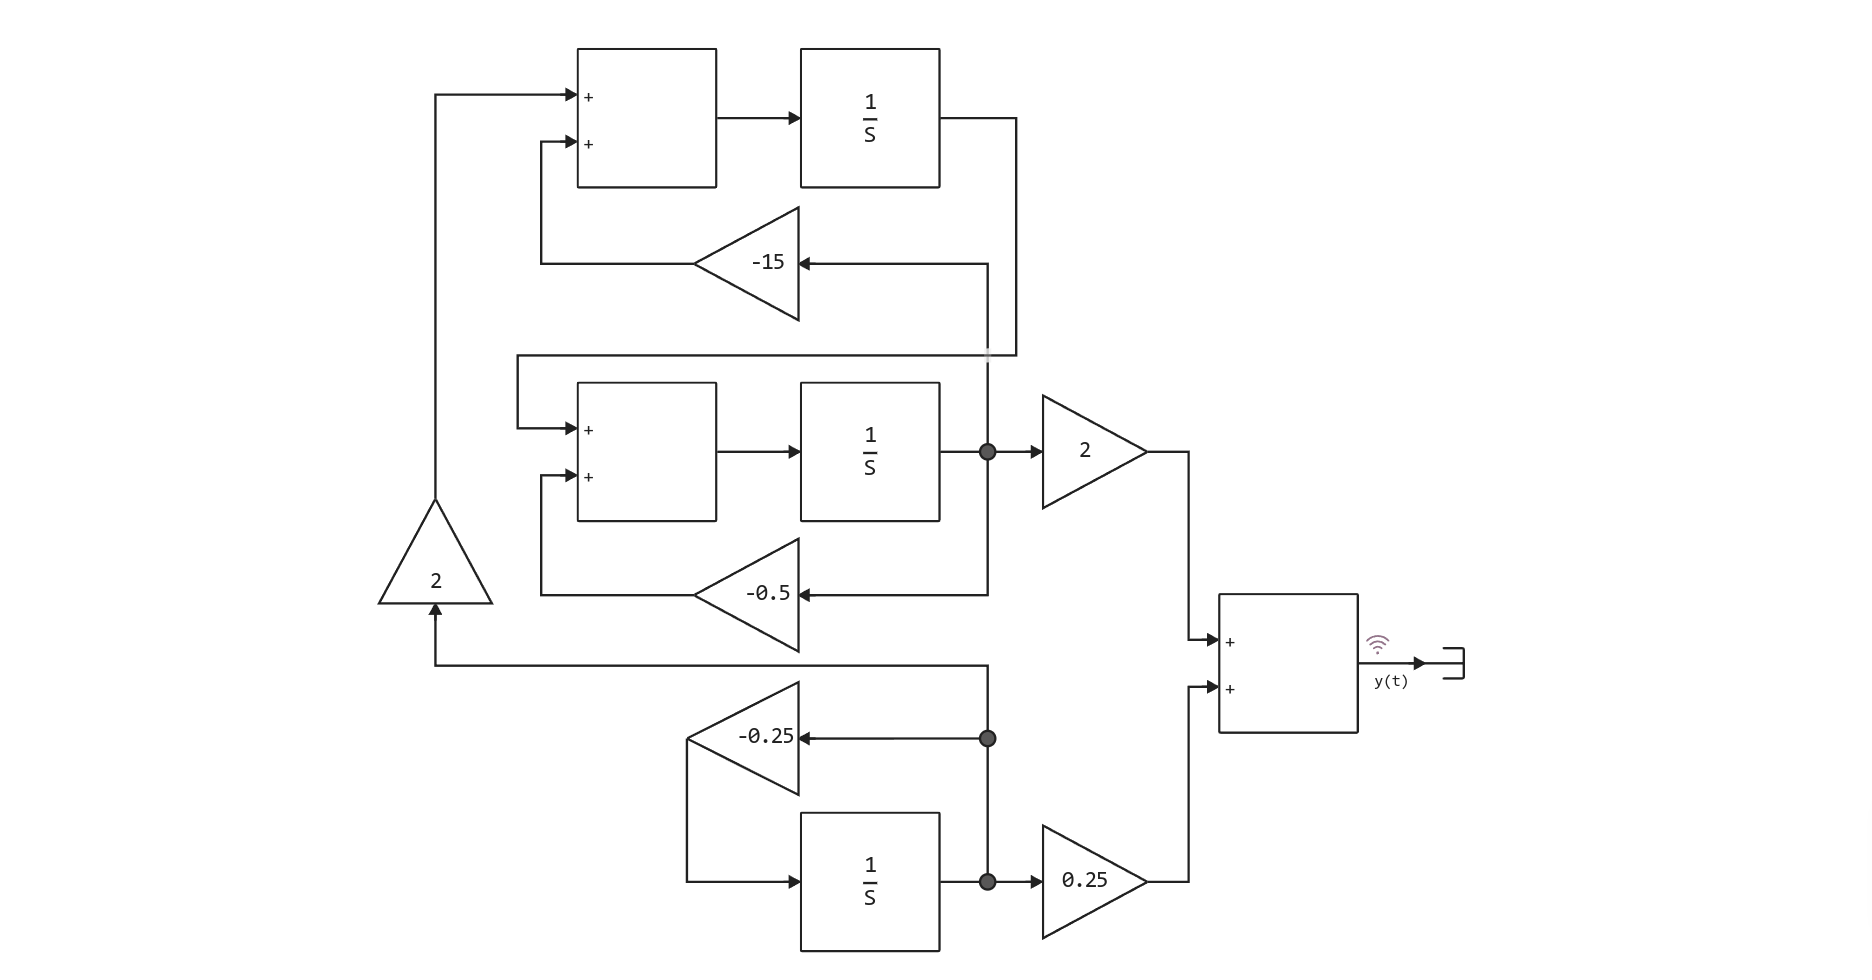
\includegraphics[height=0.27\textheight]{sources/task2_free_model.png}
    \caption*{Схема моделирования свободного движения линейной динамической системы}
\end{figure}
График $y(t)$ в таком случае будет выглядеть так:
\begin{figure}[H]
    \centering
    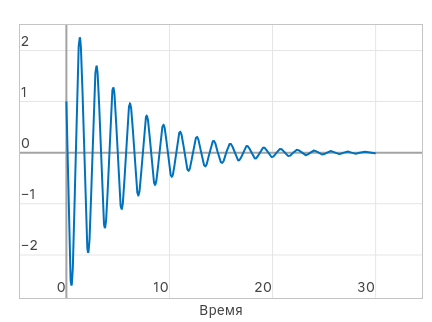
\includegraphics[width=0.4\textwidth]{sources/task2_free_y.png}
    \caption*{График $y(t)$ при свободном движении системы}
\end{figure}
\addsection{Выводы}
Благодаря моделированию линейных динамических систем как в виде скалярного дифференциального уравнения $n$-го порядка, так и в виде $n$ дифференциальных уравнений первого порядка мы ознакомились с пакетом прикладных программ Simulink и овладели основными приёмами, которые помогают моделировать такие системы.
\end{document}